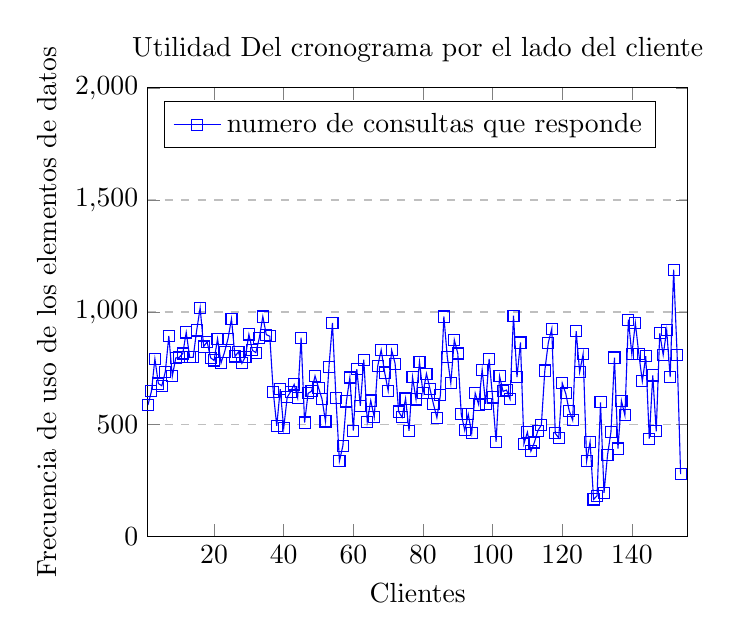
\begin{tikzpicture}
\begin{axis}[
    title={Utilidad Del cronograma por el lado del cliente},
    xlabel={Clientes},
    ylabel={Frecuencia de uso de los elementos de datos},
    xmin=1, xmax=156,
    ymin=0, ymax=2000,
    xtick={},
    ytick={},
    legend pos=north west,
    ymajorgrids=true,
    grid style=dashed,
]

\addplot[
    color=blue,
    mark=square,
    ]
    coordinates {
    %USO EXACTO
    (1,585)
(2,646)
(3,791)
(4,681)
(5,671)
(6,734)
(7,893)
(8,714)
(9,795)
(10,798)
(11,815)
(12,909)
(13,798)
(14,798)
(15,918)
(16,1019)
(17,846)
(18,867)
(19,796)
(20,784)
(21,881)
(22,773)
(23,821)
(24,881)
(25,970)
(26,802)
(27,822)
(28,771)
(29,801)
(30,900)
(31,829)
(32,819)
(33,885)
(34,980)
(35,899)
(36,892)
(37,644)
(38,492)
(39,656)
(40,482)
(41,620)
(42,645)
(43,677)
(44,618)
(45,886)
(46,507)
(47,637)
(48,647)
(49,715)
(50,662)
(51,612)
(52,512)
(53,756)
(54,952)
(55,618)
(56,335)
(57,404)
(58,601)
(59,708)
(60,471)
(61,745)
(62,582)
(63,787)
(64,511)
(65,605)
(66,531)
(67,759)
(68,831)
(69,730)
(70,649)
(71,830)
(72,770)
(73,556)
(74,530)
(75,614)
(76,470)
(77,710)
(78,610)
(79,778)
(80,638)
(81,725)
(82,658)
(83,590)
(84,529)
(85,629)
(86,980)
(87,798)
(88,683)
(89,876)
(90,815)
(91,544)
(92,472)
(93,544)
(94,459)
(95,638)
(96,587)
(97,743)
(98,590)
(99,791)
(100,619)
(101,421)
(102,714)
(103,646)
(104,652)
(105,612)
(106,984)
(107,710)
(108,864)
(109,412)
(110,464)
(111,379)
(112,418)
(113,471)
(114,496)
(115,739)
(116,863)
(117,926)
(118,459)
(119,438)
(120,683)
(121,637)
(122,560)
(123,517)
(124,915)
(125,732)
(126,813)
(127,335)
(128,421)
(129,164)
(130,180)
(131,597)
(132,193)
(133,361)
(134,466)
(135,797)
(136,391)
(137,604)
(138,539)
(139,966)
(140,811)
(141,951)
(142,813)
(143,691)
(144,803)
(145,435)
(146,717)
(147,468)
(148,905)
(149,809)
(150,919)
(151,710)
(152,1189)
(153,809)
(154,277)
    };
    \legend{numero de consultas que responde}

\end{axis}
\end{tikzpicture}

